\documentclass[border=2pt]{standalone}
\usepackage{pgfplots}
\pgfplotsset{compat=1.18}
\begin{document}
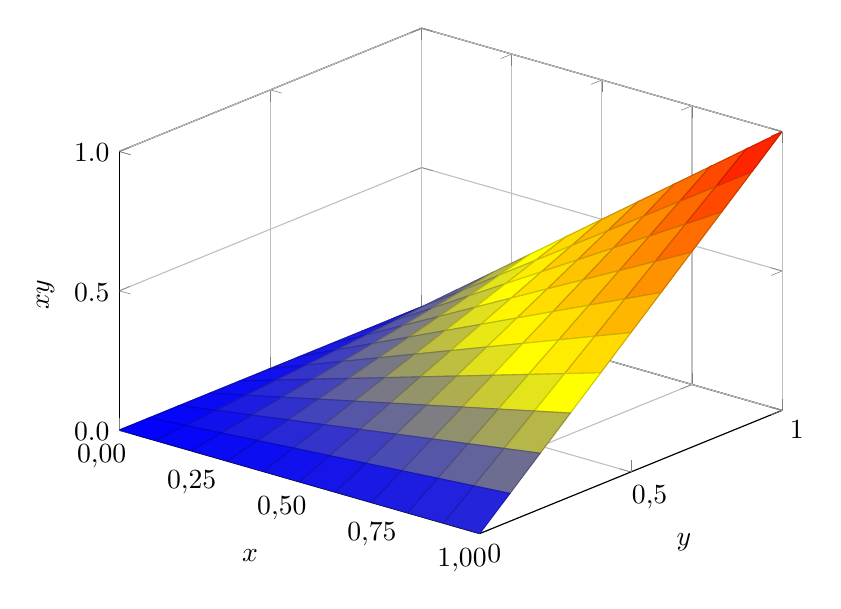
\begin{tikzpicture}
  \begin{axis}[
    width=10cm,
    height=8cm,
    view={40}{30},
    domain=0:1,
    y domain=0:1,
    samples=11,
    xmin=0,
    xmax=1,
    ymin=0,
    ymax=1,
    zmin=0,
    zmax=1,
    xtick={0,0.25,0.5,0.75,1},
    ytick={0,0.5,1},
    ztick={0,0.5,1},
    xticklabel={$\pgfmathprintnumber[fixed,fixed zerofill,precision=2,use comma]{\tick}$},
    yticklabel={$\pgfmathprintnumber[fixed,precision=2,use comma]{\tick}$},
    zticklabel={$\pgfmathprintnumber[fixed,fixed zerofill,precision=1]{\tick}$},
    grid=major,
    xlabel={$x$},
    ylabel={$y$},
    zlabel={$xy$}
  ]
    \addplot3[surf] {x*y};
  \end{axis}
\end{tikzpicture}
\end{document}
